\documentclass[11pt]{standalone}

\usepackage{helvet}
\usepackage{units}
\usepackage{textcomp}

\usepackage{ifthen}
\usepackage{tikz} 
\usetikzlibrary{shapes.misc}
\usetikzlibrary{arrows,arrows.meta}
\usetikzlibrary{calc,intersections, patterns, math}
\usetikzlibrary{decorations.pathmorphing}
\usetikzlibrary{shapes.geometric}

\definecolor{pfeil}{RGB}{168,167,167}
\definecolor{petrol}{RGB}{0, 118, 136}
\definecolor{blue}{RGB}{0, 118, 136}
\definecolor{white}{RGB}{35,35,35}
% \definecolor{blue}{RGB}{100, 100, 255}
\definecolor{darkgoldenrod}{RGB}{184, 134, 11}
\colorlet{petrol-lighter}{petrol!40}
\colorlet{darkgoldenrod-lighter}{darkgoldenrod!40}
\definecolor{background}{RGB}{35,35,35}

\begin{document}

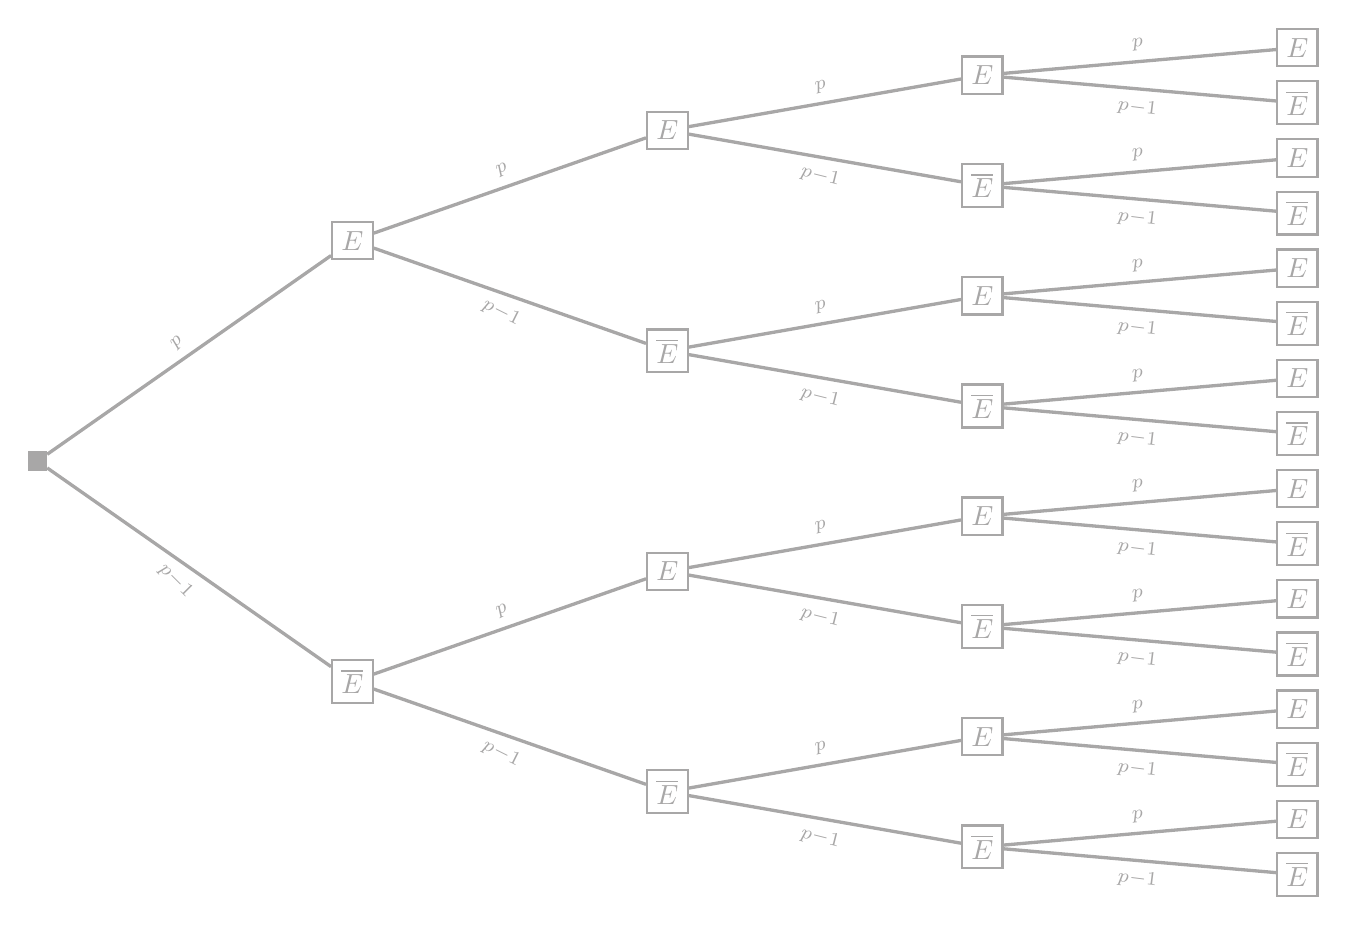
\begin{tikzpicture}[pfeil, xscale=1, yscale=0.7]

	% Stufe 1
	\node[draw,fill] (S) at (0,0) {};
	
	\node[draw,rectangle, thick] (F1) at (4,4) {$E$};
	\node[draw,rectangle, thick] (F2) at (4,-4) {$\overline E$};
	
	\draw[very thick] (S) -- node[above, sloped] {$\scriptstyle  p$} (F1);
	\draw[very thick] (S) -- node[below, sloped] {$\scriptstyle  p-1$} (F2);

	% Stufe 2
	\node[draw,rectangle, thick] (F11) at (8,6) {$E$};
	\node[draw,rectangle, thick] (F12) at (8,2) {$\overline E$};
	
	\draw[very thick] (F1) -- node[above, sloped] {$\scriptstyle p$} (F11);
	\draw[very thick] (F1) -- node[below, sloped] {$\scriptstyle p-1$} (F12);

	\node[draw,rectangle, thick] (F21) at (8,-2) {$E$};
	\node[draw,rectangle, thick] (F22) at (8,-6) {$\overline E$};
	
	\draw[very thick] (F2) -- node[above, sloped] {$\scriptstyle p$} (F21);
	\draw[very thick] (F2) -- node[below, sloped] {$\scriptstyle p-1$} (F22);

	% Stufe 3
	\node[draw,rectangle, thick] (F111) at (12,7) {$E$};
	\node[draw,rectangle, thick] (F112) at (12,5) {$\overline E$};
	
	\draw[very thick] (F11) -- node[above, sloped] {$\scriptstyle p$} (F111);
	\draw[very thick] (F11) -- node[below, sloped] {$\scriptstyle p-1$} (F112);		

	\node[draw,rectangle, thick] (F121) at (12,3) {$E$};
	\node[draw,rectangle, thick] (F122) at (12,1) {$\overline E$};
	
	\draw[very thick] (F12) -- node[above, sloped] {$\scriptstyle p$} (F121);
	\draw[very thick] (F12) -- node[below, sloped] {$\scriptstyle p-1$} (F122);	

	\node[draw,rectangle, thick] (F211) at (12,-1) {$E$};
	\node[draw,rectangle, thick] (F212) at (12,-3) {$\overline E$};
	
	\draw[very thick] (F21) -- node[above, sloped] {$\scriptstyle p$} (F211);
	\draw[very thick] (F21) -- node[below, sloped] {$\scriptstyle p-1$} (F212);

	\node[draw,rectangle, thick] (F221) at (12,-5) {$E$};
	\node[draw,rectangle, thick] (F222) at (12,-7) {$\overline E$};
	
	\draw[very thick] (F22) -- node[above, sloped] {$\scriptstyle p$} (F221);
	\draw[very thick] (F22) -- node[below, sloped] {$\scriptstyle p-1$} (F222);

	% Stufe 4
	\node[draw,rectangle, thick] (F1111) at (16,7.5) {$E$};
	\node[draw,rectangle, thick] (F1112) at (16,6.5) {$\overline E$};
	
	\draw[very thick] (F111) -- node[above, sloped] {$\scriptstyle p$} (F1111);
	\draw[very thick] (F111) -- node[below, sloped] {$\scriptstyle p-1$} (F1112);	
	
	\node[draw,rectangle, thick] (F1121) at (16,5.5) {$E$};
	\node[draw,rectangle, thick] (F1122) at (16,4.5) {$\overline E$};
	
	\draw[very thick] (F112) -- node[above, sloped] {$\scriptstyle p$} (F1121);
	\draw[very thick] (F112) -- node[below, sloped] {$\scriptstyle p-1$} (F1122);
	
	\node[draw,rectangle, thick] (F1211) at (16,3.5) {$E$};
	\node[draw,rectangle, thick] (F1212) at (16,2.5) {$\overline E$};
	
	\draw[very thick] (F121) -- node[above, sloped] {$\scriptstyle p$} (F1211);
	\draw[very thick] (F121) -- node[below, sloped] {$\scriptstyle p-1$} (F1212);	
	
	\node[draw,rectangle, thick] (F1221) at (16,1.5) {$E$};
	\node[draw,rectangle, thick] (F1222) at (16,0.5) {$\overline E$};
	
	\draw[very thick] (F122) -- node[above, sloped] {$\scriptstyle p$} (F1221);
	\draw[very thick] (F122) -- node[below, sloped] {$\scriptstyle p-1$} (F1222);


	\node[draw,rectangle, thick] (F2111) at (16,-0.5) {$E$};
	\node[draw,rectangle, thick] (F2112) at (16,-1.5) {$\overline E$};
	
	\draw[very thick] (F211) -- node[above, sloped] {$\scriptstyle p$} (F2111);
	\draw[very thick] (F211) -- node[below, sloped] {$\scriptstyle p-1$} (F2112);	
	
	\node[draw,rectangle, thick] (F2121) at (16,-2.5) {$E$};
	\node[draw,rectangle, thick] (F2122) at (16,-3.5) {$\overline E$};
	
	\draw[very thick] (F212) -- node[above, sloped] {$\scriptstyle p$} (F2121);
	\draw[very thick] (F212) -- node[below, sloped] {$\scriptstyle p-1$} (F2122);
	
	\node[draw,rectangle, thick] (F2211) at (16,-4.5) {$E$};
	\node[draw,rectangle, thick] (F2212) at (16,-5.5) {$\overline E$};
	
	\draw[very thick] (F221) -- node[above, sloped] {$\scriptstyle p$} (F2211);
	\draw[very thick] (F221) -- node[below, sloped] {$\scriptstyle p-1$} (F2212);	
	
	\node[draw,rectangle, thick] (F2221) at (16,-6.5) {$E$};
	\node[draw,rectangle, thick] (F2222) at (16,-7.5) {$\overline E$};
	
	\draw[very thick] (F222) -- node[above, sloped] {$\scriptstyle p$} (F2221);
	\draw[very thick] (F222) -- node[below, sloped] {$\scriptstyle p-1$} (F2222);
\end{tikzpicture}




\end{document}
